% Options for packages loaded elsewhere
% Options for packages loaded elsewhere
\PassOptionsToPackage{unicode}{hyperref}
\PassOptionsToPackage{hyphens}{url}
\PassOptionsToPackage{dvipsnames,svgnames,x11names}{xcolor}
%
\documentclass[
  letterpaper,
  DIV=11,
  numbers=noendperiod]{scrartcl}
\usepackage{xcolor}
\usepackage{amsmath,amssymb}
\setcounter{secnumdepth}{-\maxdimen} % remove section numbering
\usepackage{iftex}
\ifPDFTeX
  \usepackage[T1]{fontenc}
  \usepackage[utf8]{inputenc}
  \usepackage{textcomp} % provide euro and other symbols
\else % if luatex or xetex
  \usepackage{unicode-math} % this also loads fontspec
  \defaultfontfeatures{Scale=MatchLowercase}
  \defaultfontfeatures[\rmfamily]{Ligatures=TeX,Scale=1}
\fi
\usepackage{lmodern}
\ifPDFTeX\else
  % xetex/luatex font selection
\fi
% Use upquote if available, for straight quotes in verbatim environments
\IfFileExists{upquote.sty}{\usepackage{upquote}}{}
\IfFileExists{microtype.sty}{% use microtype if available
  \usepackage[]{microtype}
  \UseMicrotypeSet[protrusion]{basicmath} % disable protrusion for tt fonts
}{}
\makeatletter
\@ifundefined{KOMAClassName}{% if non-KOMA class
  \IfFileExists{parskip.sty}{%
    \usepackage{parskip}
  }{% else
    \setlength{\parindent}{0pt}
    \setlength{\parskip}{6pt plus 2pt minus 1pt}}
}{% if KOMA class
  \KOMAoptions{parskip=half}}
\makeatother
% Make \paragraph and \subparagraph free-standing
\makeatletter
\ifx\paragraph\undefined\else
  \let\oldparagraph\paragraph
  \renewcommand{\paragraph}{
    \@ifstar
      \xxxParagraphStar
      \xxxParagraphNoStar
  }
  \newcommand{\xxxParagraphStar}[1]{\oldparagraph*{#1}\mbox{}}
  \newcommand{\xxxParagraphNoStar}[1]{\oldparagraph{#1}\mbox{}}
\fi
\ifx\subparagraph\undefined\else
  \let\oldsubparagraph\subparagraph
  \renewcommand{\subparagraph}{
    \@ifstar
      \xxxSubParagraphStar
      \xxxSubParagraphNoStar
  }
  \newcommand{\xxxSubParagraphStar}[1]{\oldsubparagraph*{#1}\mbox{}}
  \newcommand{\xxxSubParagraphNoStar}[1]{\oldsubparagraph{#1}\mbox{}}
\fi
\makeatother


\usepackage{longtable,booktabs,array}
\usepackage{calc} % for calculating minipage widths
% Correct order of tables after \paragraph or \subparagraph
\usepackage{etoolbox}
\makeatletter
\patchcmd\longtable{\par}{\if@noskipsec\mbox{}\fi\par}{}{}
\makeatother
% Allow footnotes in longtable head/foot
\IfFileExists{footnotehyper.sty}{\usepackage{footnotehyper}}{\usepackage{footnote}}
\makesavenoteenv{longtable}
\usepackage{graphicx}
\makeatletter
\newsavebox\pandoc@box
\newcommand*\pandocbounded[1]{% scales image to fit in text height/width
  \sbox\pandoc@box{#1}%
  \Gscale@div\@tempa{\textheight}{\dimexpr\ht\pandoc@box+\dp\pandoc@box\relax}%
  \Gscale@div\@tempb{\linewidth}{\wd\pandoc@box}%
  \ifdim\@tempb\p@<\@tempa\p@\let\@tempa\@tempb\fi% select the smaller of both
  \ifdim\@tempa\p@<\p@\scalebox{\@tempa}{\usebox\pandoc@box}%
  \else\usebox{\pandoc@box}%
  \fi%
}
% Set default figure placement to htbp
\def\fps@figure{htbp}
\makeatother


% definitions for citeproc citations
\NewDocumentCommand\citeproctext{}{}
\NewDocumentCommand\citeproc{mm}{%
  \begingroup\def\citeproctext{#2}\cite{#1}\endgroup}
\makeatletter
 % allow citations to break across lines
 \let\@cite@ofmt\@firstofone
 % avoid brackets around text for \cite:
 \def\@biblabel#1{}
 \def\@cite#1#2{{#1\if@tempswa , #2\fi}}
\makeatother
\newlength{\cslhangindent}
\setlength{\cslhangindent}{1.5em}
\newlength{\csllabelwidth}
\setlength{\csllabelwidth}{3em}
\newenvironment{CSLReferences}[2] % #1 hanging-indent, #2 entry-spacing
 {\begin{list}{}{%
  \setlength{\itemindent}{0pt}
  \setlength{\leftmargin}{0pt}
  \setlength{\parsep}{0pt}
  % turn on hanging indent if param 1 is 1
  \ifodd #1
   \setlength{\leftmargin}{\cslhangindent}
   \setlength{\itemindent}{-1\cslhangindent}
  \fi
  % set entry spacing
  \setlength{\itemsep}{#2\baselineskip}}}
 {\end{list}}
\usepackage{calc}
\newcommand{\CSLBlock}[1]{\hfill\break\parbox[t]{\linewidth}{\strut\ignorespaces#1\strut}}
\newcommand{\CSLLeftMargin}[1]{\parbox[t]{\csllabelwidth}{\strut#1\strut}}
\newcommand{\CSLRightInline}[1]{\parbox[t]{\linewidth - \csllabelwidth}{\strut#1\strut}}
\newcommand{\CSLIndent}[1]{\hspace{\cslhangindent}#1}



\setlength{\emergencystretch}{3em} % prevent overfull lines

\providecommand{\tightlist}{%
  \setlength{\itemsep}{0pt}\setlength{\parskip}{0pt}}



 


\KOMAoption{captions}{tableheading}
\makeatletter
\@ifpackageloaded{caption}{}{\usepackage{caption}}
\AtBeginDocument{%
\ifdefined\contentsname
  \renewcommand*\contentsname{Table of contents}
\else
  \newcommand\contentsname{Table of contents}
\fi
\ifdefined\listfigurename
  \renewcommand*\listfigurename{List of Figures}
\else
  \newcommand\listfigurename{List of Figures}
\fi
\ifdefined\listtablename
  \renewcommand*\listtablename{List of Tables}
\else
  \newcommand\listtablename{List of Tables}
\fi
\ifdefined\figurename
  \renewcommand*\figurename{Figure}
\else
  \newcommand\figurename{Figure}
\fi
\ifdefined\tablename
  \renewcommand*\tablename{Table}
\else
  \newcommand\tablename{Table}
\fi
}
\@ifpackageloaded{float}{}{\usepackage{float}}
\floatstyle{ruled}
\@ifundefined{c@chapter}{\newfloat{codelisting}{h}{lop}}{\newfloat{codelisting}{h}{lop}[chapter]}
\floatname{codelisting}{Listing}
\newcommand*\listoflistings{\listof{codelisting}{List of Listings}}
\makeatother
\makeatletter
\makeatother
\makeatletter
\@ifpackageloaded{caption}{}{\usepackage{caption}}
\@ifpackageloaded{subcaption}{}{\usepackage{subcaption}}
\makeatother
\usepackage{bookmark}
\IfFileExists{xurl.sty}{\usepackage{xurl}}{} % add URL line breaks if available
\urlstyle{same}
\hypersetup{
  pdftitle={Binary Classification of Hotel Cancellations},
  pdfauthor={Ashifa Hassam, Nour Shawky, Athul Sasidharan, Kin Chung Choy},
  colorlinks=true,
  linkcolor={blue},
  filecolor={Maroon},
  citecolor={Blue},
  urlcolor={Blue},
  pdfcreator={LaTeX via pandoc}}


\title{Binary Classification of Hotel Cancellations}
\author{Ashifa Hassam, Nour Shawky, Athul Sasidharan, Kin Chung Choy}
\date{}
\begin{document}
\maketitle

\renewcommand*\contentsname{Table of contents}
{
\hypersetup{linkcolor=}
\setcounter{tocdepth}{3}
\tableofcontents
}

\subsection{Summary}\label{summary}

In this project we worked with an open hotel booking dataset containing
reservations for both city and resort hotels and we selected a smaller
set of features that would realistically be available at the time of
booking, such as lead time, whether the guest is a repeat customer,
previous cancellations, booking changes, special requests, reserved room
type and deposit type. After a brief exploratory analysis, we confirmed
that cancellations are fairly common and that patterns differ across
hotel types and booking conditions, especially for repeated guests and
deposit policies. We then framed the problem as a binary classification
task: predict whether a booking will be cancelled or not. The data was
split into training and test sets, and we built pipelines that combined
preprocessing with three models: K-Nearest Neighbours, a Decision Tree
and an RBF-kernel SVM.

Using 5-fold cross validation with F1 score on the validation set, KNN
gave the best performance, so we chose it as our final model and
evaluated it on the unseen test data. On the test set, our KNN model
performs well enough with an accuracy of 73\% and we concluded that it
could plausibly support day-to-day hotel operations, at least as a
first-pass tool for flagging higher-risk bookings. The confusion matrix
shows that the model correctly identifies most non-cancellations and
captures a reasonable portion of true cancellations, even though it
still misses some risky bookings. That said, we do not see it as a
finished solution. There is clear value in extending the feature set,
tuning the model more carefully, and examining in detail which types of
reservations are consistently mis-classified. This would not only
improve raw performance, but also give hotels a better sense of when to
rely on the model's predictions and when they should be treated as one
input alongside staff experience and existing booking policies.

\subsection{Introduction}\label{introduction}

Free cancellations for hotel bookings are increasingly popular nowadays,
but cancellations create significant impact on a hotel's revenue and
operation. Predicting whether a reservation will be canceled can help
hotels manage resources more effectively, reduce lost revenue, and
improve customer service. There has been a rise in the research
conducted on predicting hotel cancellations using machine learning
models in order to improve strategies for revenue management (Sánchez,
Sánchez-Medina, and Pellejero 2020; Antonio, Almeida, and Nunes 2017).
In our project, we aim to answer the question ``Can we build a model
that accurately predicts whether a hotel booking will be canceled?''
This will be a binary classification problem, where each booking is
labeled as either ``canceled'' or ``not canceled''.

To explore this, we used a publicly available dataset from
\href{https://raw.githubusercontent.com/manthangandhi/hotel_cancellation_prediction/refs/heads/main/data/hotel_bookings.csv}{GitHub}.
The dataset contains information about hotel reservations, and the label
column is called ``IsCanceled'', which indicates whether a booking was
canceled or not. One of the important features is ``Lead Time'', showing
how many days passed between the booking date and the arrival date. Some
other important features include deposit type, is\_repeated\_guest and
booking\_changes, which are all helpful for our classification model and
have been used in previous work done that has also conducted predictive
modeling on hotel cancelations (Antonio, Almeida, and Nunes 2019).

\subsection{Question of Interest}\label{question-of-interest}

Since the dataset contains many features (32 in total), we chose to
examine a subset of these in order to focus our research question to the
following: \textbf{Can we predict hotel cancellations from booking lead
time and different types of guest behaviors, using hotel booking
information from the year 2017? And do cancellations differ across hotel
type?}

\subsection{Methods}\label{methods}

\subsection{Data}\label{data}

We began by cleaning the dataset and selecting the columns that we
considered most useful for our research question. Our analysis depends
on the following columns as predictors: hotel, is\_canceled, lead\_time,
previous\_cancellations,previous\_bookings\_not\_canceled,
booking\_changes,total\_of\_special\_requests, is\_repeated\_guest,
deposit\_type and reserved\_room\_type.

To ensure quality and integrity of the data prior to modelling, we used
the pandera package to conduct a series of validation checks. These
checks enforced correct column name and column types, valid category
levels and numerical bounds for our predictor variables. We then
performed exploratory data analysis (EDA) to examine the distribution of
our predictor variables across different levels of our target variable,
`is\_canceled'.

For predictive modeling, we conducted cross validation on 3 different
models: KNN, SVM RBF and Decision trees, using our training data. The
best performing model (KNN) was then evaluated on the test set to assess
whether it generalizes well to unseen data and evaluate how well it was
able to correctly predict guests that cancel their hotel reservations
versus those who do not.Since the entire dataset is quite large, we'll
be focusing on hotel data from the most recent year, the year 2017, to
make predictions about hotel cancellations (as per the research
question).

\subsection{Analysis}\label{analysis}

The correlation matrix (Figure~\ref{fig-corrmatrix}) helped us assess
how our selected numerical features relate to one another and to the
target variable, is\_canceled. Overall, the matrix shows that most
predictors have only weak linear relationships with cancellations, which
suggests that no single booking feature is strongly determinant on its
own. This aligns with our expectation that cancellation behavior is
influenced by several interacting factors rather than a single dominant
one. We do, however, observe some stronger correlations among the guest
history features: lead\_time, previous\_cancellations, and
previous\_bookings\_not\_canceled are highly related, reflecting that
guests with long booking horizons tend to be more frequent travelers
with greater booking histories. These relationships are not necessarily
indicative of cancellation risk themselves, but they confirmed that our
predictor set contains overlapping behavioral signals that the model
will need to note.

\begin{figure}

\centering{

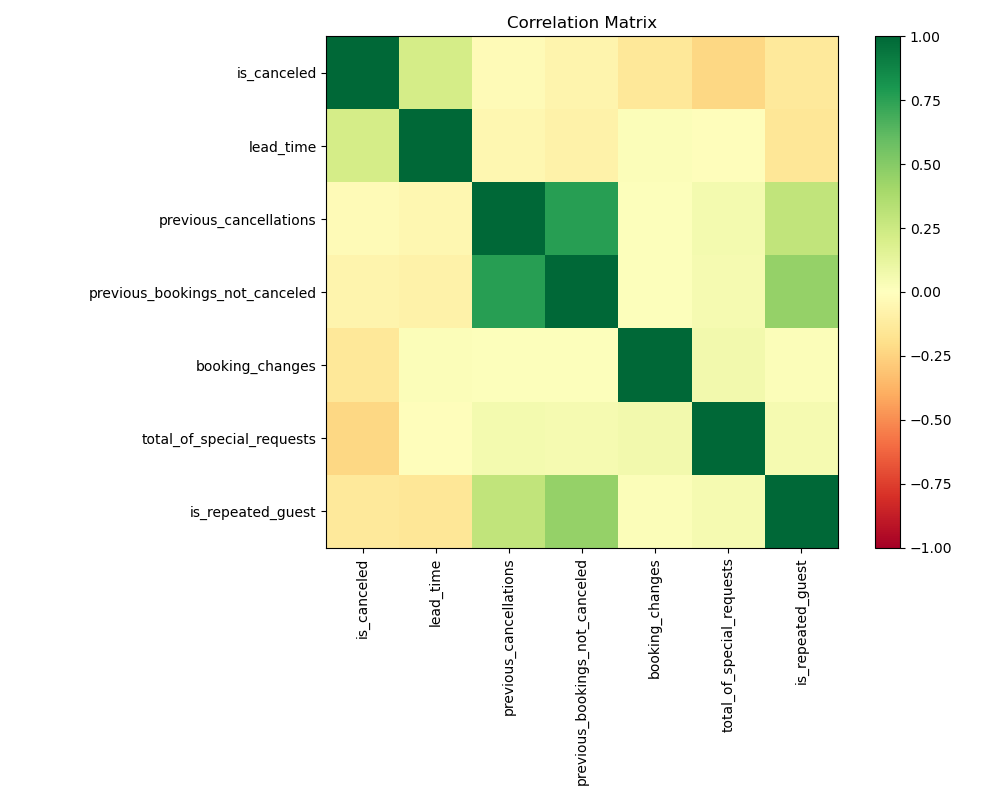
\includegraphics[width=0.7\linewidth,height=\textheight,keepaspectratio]{../results/figures/eda_correlation_matrix.png}

}

\caption{\label{fig-corrmatrix}Correlation Matrix of Selected Numerical
Features.}

\end{figure}%

We can observe from Figure~\ref{fig-eda-bars} that almost all
cancellations are happening for new guests. Repeated guests who have
previously booked with the hotel before do not seem to cancel much. In
addition, the majority of cancellations occur for guests who have booked
room type A. Interestingly, guests seem to cancel more when they have
not provided a deposit on their booking and some also cancel when their
deposit is non refundable.

One small but notable pattern is the slight negative correlation between
total\_of\_special\_requests and is\_canceled, suggesting that guests
who invest more effort in customizing their stay may be somewhat less
likely to cancel. Although this relationship is modest, it supports our
decision to include special requests in the feature set, as even weak
signals can help a classification model refine its decision boundary.
Similarly, mild positive correlations between lead\_time and
is\_canceled indicate that far-in-advance bookings tend to cancel
slightly more often, a trend also reported in the hotel cancellation
literature (Antonio, De Almeida, and Nunes 2019; Antonio, Almeida, and
Nunes 2019).

\begin{figure}

\centering{

\begin{minipage}{0.32\linewidth}
\centering
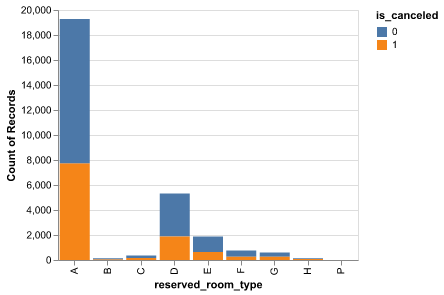
\includegraphics[width=\linewidth]{../results/figures/eda_reserved_room_type_vs_cancellations.png}
\end{minipage}
\hfill
\begin{minipage}{0.32\linewidth}
\centering
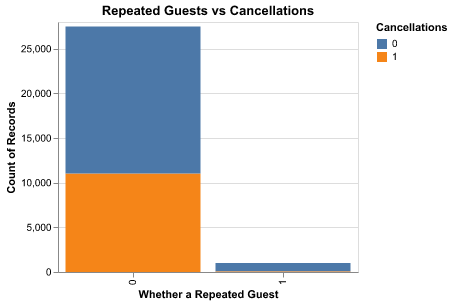
\includegraphics[width=\linewidth]{../results/figures/eda_repeated_guest_vs_cancellations_count.png}
\end{minipage}
\hfill
\begin{minipage}{0.32\linewidth}
\centering
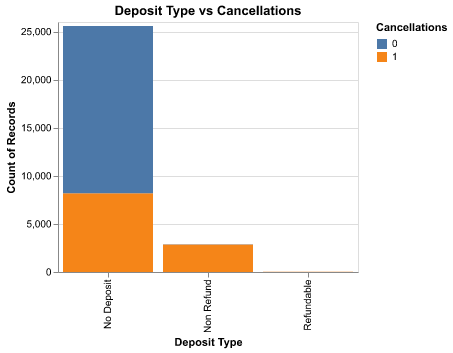
\includegraphics[width=\linewidth]{../results/figures/eda_deposit_type_vs_cancellations_count.png}
\end{minipage}

}

\caption{\label{fig-eda-bars}EDA bar plots: Reserved Room Type, Repeated
Guest Status, and Deposit Type vs Cancellations.}

\end{figure}%

\subsection{Discussion of Results}\label{discussion-of-results}

With this project, our primary goal was to predict the whether a hotel
booking would eventually end up being cancelled, using information that
is available at the time of booking including lead time, deposit type,
room type and whether the guest is a repeat customer etc. The idea is
that a reasonably accurate model could help hotel businesses flag
high-risk bookings and adjust their policies or communication before the
stay date.

For the purpose of getting the best model to do this prediction, we
compared three classification models using 5-fold cross validation on
the training set, with F1 score (for the cancellation class) as the main
metric, \textbf{K-Nearest Neighbours (KNN, k = 15), Decision Tree
(max\_depth = 6), and RBF-kernel SVM (C = 1.0, gamma = ``scale'').}
After scoring their mean F1 scores on the training folds, the F1 score
results were: F1 = 0.602 for KNN, F1= 0.57 for Decision Tree and
F1=0.526 for RBF SVM. KNN clearly performed best on this metric, and
also consistently across the folds with the least standard deviations.
Because our main concern is to correctly identify cancellations rather
than just overall accuracy, we chose \textbf{KNN} as the final model for
evaluation on the test set.

\begin{figure}

\centering{

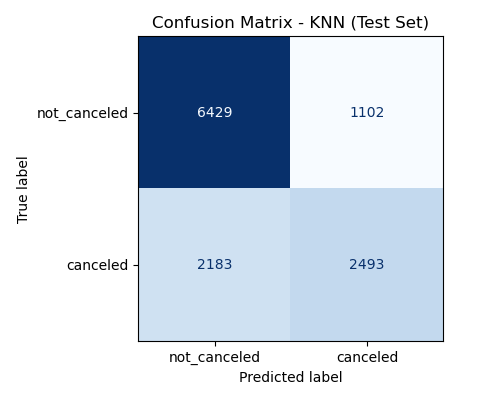
\includegraphics[width=0.7\linewidth,height=\textheight,keepaspectratio]{../results/figures/confusion_matrix_knn.png}

}

\caption{\label{fig-knnconfusion}KNN Confusion Matrix}

\end{figure}%

As shown in Figure Figure~\ref{fig-knnconfusion}, the KNN model achieved
an accuracy of 0.732. Other stats are as follows:

\begin{itemize}
\tightlist
\item
  Cancellation Precision ≈ 0.70
\item
  Cancellation Recall ≈ 0.53
\item
  Cancellation F1 ≈ 0.60
\item
  Non-Cancellation Precision ≈ 0.75
\item
  Non-Cancellation Recall ≈ 0.86
\item
  Non-Cancellation F1 ≈ 0.80
\end{itemize}

The averaged F1 is close to 0.70, which is close to what we saw in the
cross validation for the cancellation class. This suggests that the
model do generally well enough and does not drastically overfit the
training data.

If we assume a rough baseline of always predicting ``not cancelled'',
the model would give an accuracy of 62\%. So looking into that, our KNN
model improves this by about 73\% which also provides a meaningful
recall for the cancellation class. Our model leans slightly towards
being a bit cautious about over-flagging cancellations (higher position
than recall for positive class). But in practice, this is acceptable, as
the hotel would want to avoid annoying, loyal and serious guests with
extra checks, but it also would be very useful in catching more of these
genuinely risky bookings.

\begin{figure}

\centering{

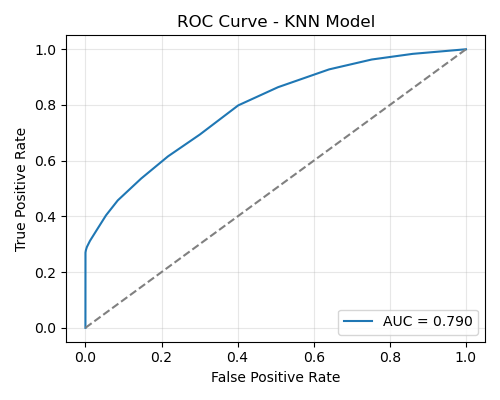
\includegraphics[width=0.7\linewidth,height=\textheight,keepaspectratio]{../results/figures/roc_curve_knn.png}

}

\caption{\label{fig-knnroc}ROC Curve for the KNN Model}

\end{figure}%

The ROC curve for the KNN model, Figure~\ref{fig-knnroc}, shows how well
the classifier can distinguish between cancelled and non-cancelled
bookings across all possible classification thresholds. The curve rises
well above the diagonal baseline, indicating that the model performs
substantially better than random guessing. At lower false positive
rates, the true positive rate increases steadily, suggesting that the
model can identify a meaningful proportion of cancellations even when
constrained to make very few false alarms. The curve becomes steeper as
the threshold relaxes, reflecting that the model captures more
cancellations at the cost of some additional false positives---a
trade-off that is expected in this type of classification problem.

The AUC value of 0.79 provides a concise summary of this performance. An
AUC of 0.79 indicates good discriminatory ability, meaning that in
roughly 79\% of random pairings between a canceled and a non-canceled
booking, the model assigns a higher cancellation probability to the
canceled booking. Although this is not exceptionally high, it is
noticeably stronger than a naive baseline and aligns with the F1 and
accuracy scores observed in earlier evaluations. Overall, the ROC curve
reinforces that the KNN model captures meaningful patterns in guest
behavior and booking characteristics, even though there remains room to
improve its ability to detect more of the truly high-risk cancellations.

\textbf{Limitations to keep in mind when interpreting :}

\begin{itemize}
\tightlist
\item
  \textbf{Feature and dataset limitations:} The dataset has restricted
  us with booking data from only one year - 2017, and also it is taken
  from a mix for too many countries. This simplifies the problem but may
  limit how well the model generalizes to other years with different
  travel patterns or external events. The analysis might differ from
  location to location and country to country. We used a small, curated
  set of features thus including more information (such as market
  segment, distribution channel, length of stay or country) could help
  the model learn more subtle patterns and improve recall for
  cancellations.
\item
  \textbf{No hyperparameter tuning yet:} We used fixed hyperparameters
  (e.g., k = 15 for KNN) rather than performing a grid search or
  randomized search. Systematic tuning could yield a better balance
  between precision and recall for the cancellation class.
\item
  \textbf{Single threshold:} We used the default decision threshold of
  0.5. For a real hotel, it might be better to adjust this threshold
  depending on whether they are more concerned about missed
  cancellations or about over-flagging guests.
\end{itemize}

\textbf{Overall takeaway:}

In overall, the KNN model provides a \textbf{useful starting point} for
predicting hotel booking cancellations. It clearly outperforms a simple
majority baseline, correctly identifies most non-cancellations and
captures a meaningful portion of actual cancellations. With additional
tuning, more features and a more careful treatment of missing values and
thresholds, this approach could be developed into a practical decision
support tool to help hotels manage overbooking strategies, communicate
proactively with high-risk guests and reduce the last minute revenue
losses.

\subsection*{References}\label{references}
\addcontentsline{toc}{subsection}{References}

\phantomsection\label{refs}
\begin{CSLReferences}{1}{0}
\bibitem[\citeproctext]{ref-antonio2017}
Antonio, N., A. de Almeida, and L. Nunes. 2017. {``Predicting Hotel
Bookings Cancellation with a Machine Learning Classification Model.''}
In \emph{Proceedings of the 2017 16th IEEE International Conference on
Machine Learning and Applications (ICMLA)}, 1049--54. IEEE.

\bibitem[\citeproctext]{ref-antonio2019_dataset}
---------. 2019. {``Hotel Booking Demand Datasets.''} \emph{Data in
Brief} 22: 41--49.

\bibitem[\citeproctext]{ref-antonio2019_bigdata}
Antonio, N., A. De Almeida, and L. Nunes. 2019. {``Big Data in Hotel
Revenue Management: Exploring Cancellation Drivers to Gain Insights into
Booking Cancellation Behavior.''} \emph{Cornell Hospitality Quarterly}
60 (4): 298--319.

\bibitem[\citeproctext]{ref-sanchez2020}
Sánchez, E. C., A. J. Sánchez-Medina, and M. Pellejero. 2020.
{``Identifying Critical Hotel Cancellations Using Artificial
Intelligence.''} \emph{Tourism Management Perspectives} 35.

\end{CSLReferences}




\end{document}
